\documentclass[12pt]{article}

% TEMPLATE DEFAULT PACKAGES
\usepackage{amssymb,amsmath,amsfonts,eurosym,geometry,ulem,graphicx,color,setspace,sectsty,comment,natbib,pdflscape,array,adjustbox}

% ADDED PACKAGES FOR THIS MANUSCRIPT
\usepackage{palatino,newtxmath,multirow,titlesec,threeparttable,tabu,booktabs,titlesec,threeparttable,mathtools,bm,bbm,subcaption,pdflscape,tcolorbox,mathrsfs}
% endfloat,

\usepackage{afterpage}
\usepackage[hyphens]{url}
\usepackage[margin=1cm]{caption}

\usepackage[draft]{hyperref}
\newcommand{\tim}{$\,\times\,$}
% FIGURES & TABLES CAPTION STYLING
\captionsetup[figure]{labelfont={bf},name={Figure},labelsep=period}
\captionsetup[table]{labelfont={bf},name={Table},labelsep=period}

% SECTION TITLE SETTINGS
\titlelabel{\thetitle.\enskip}
\titleformat*{\section}{\large\bfseries}
\titleformat*{\subsection}{\normalsize\bfseries}

% COLUMN TYPES
\newcolumntype{L}[1]{>{\raggedright\let\newline\\\arraybackslash\hspace{0pt}}m{#1}}
\newcolumntype{C}{>{\centering\arraybackslash}p{5.2em}}
\newcolumntype{D}{>{\centering\arraybackslash}p{5em}}
\newcolumntype{R}[1]{>{\raggedleft\let\newline\\\arraybackslash\hspace{0pt}}m{#1}}


% MARGINS AND SPACING
\normalem
\geometry{left=1.1in,right=1.1in,top=1.0in,bottom=1.0in}
\setlength{\parskip}{2.5pt}

% SPECIAL CELL 
\newcommand{\specialcell}[2][c]{%
	\begin{tabular}[#1]{@{}l@{}}#2\end{tabular}}

% NO INDENT ON FOOTNOTES
\usepackage[hang,flushmargin]{footmisc}

\begin{document}



\vspace{0mm}
\begin{table}[h!]
\centering
\caption{Housing Project Areas Description}\label{table:projectdescriptives}
\vspace{0mm}
\begin{tabular}{l*{1}{cccccc}}
\toprule
  & \multicolumn{2}{c}{\textbf{All}}& \multicolumn{2}{c}{\textbf{Greenfield}}  & \multicolumn{2}{c}{\textbf{In-Situ}}   \\
  &Const. & Unconst. &Const. & Unconst.   & Const. & Unconst. \\
\midrule
 Number of Projects  & 172  & 145  & 43  & 20  & 27  & 29  \\ 
 Area (km2)  & 1.17  & 1.16  & 1.72  & 2.42  & 1.50  & 0.88  \\ 
 Median Construction Yr.  & 2006  & 2006  & 2006  & 2005  & 2004  & 2006  \\ 
 Delivered Houses  & 374  & 11  & 568  & 24  & 702  & 20  \\ 
 House Price in 1 km (R$^\dagger$)  & 188,441  & 218,635  & 194,214  & 186,841  & 179,596  & 208,570  \\ 
 Distance to CBD$^\ddagger$ (km)  & 32.5  & 27.7  & 40.5  & 39.9  & 32.6  & 30.6  \\ 

\bottomrule
\multicolumn{7}{l}{\scriptsize Const. refers to constructed projects and unconst. refers to unconstructed projects.}\\[-.5em]
\multicolumn{7}{l}{\scriptsize $^*$Calculated from {\it expected} completion dates using Gauteng National Treasury budget reports.}\\[-.5em]
\multicolumn{7}{l}{\scriptsize $^\dagger$ The USD averaged to about 7.70 Rands during the 2001-2011 period.}\\[-.5em]
\multicolumn{7}{l}{\scriptsize $^\ddagger$Measured as the average minimum distance with respect to Johannesburg and Pretoria CBDs. } \\[-.5em]
%\multicolumn{7}{l}{\scriptsize City includes projects whose centroids are within 30.4 km of their nearest CBD.} \\[-.5em]
%\multicolumn{7}{l}{\scriptsize Suburb includes projects whose centroids are further than 30.4 km from their nearest CBD.}
\end{tabular}
\end{table} 



\begin{figure*}
        \centering
   %     \caption[ Pre-Period Housing Densities in Constructed and Unconstructed Projects Areas ]
  %      {\small Pre-Period Densities} 
        %\vspace{2mm}
        \begin{subfigure}[b]{0.48\textwidth}
                    \caption[Network2]%
            {{\footnotesize \textbf{All Projects} pre-period formal raw data}}    
            \label{fig:prefor}
            \centering
            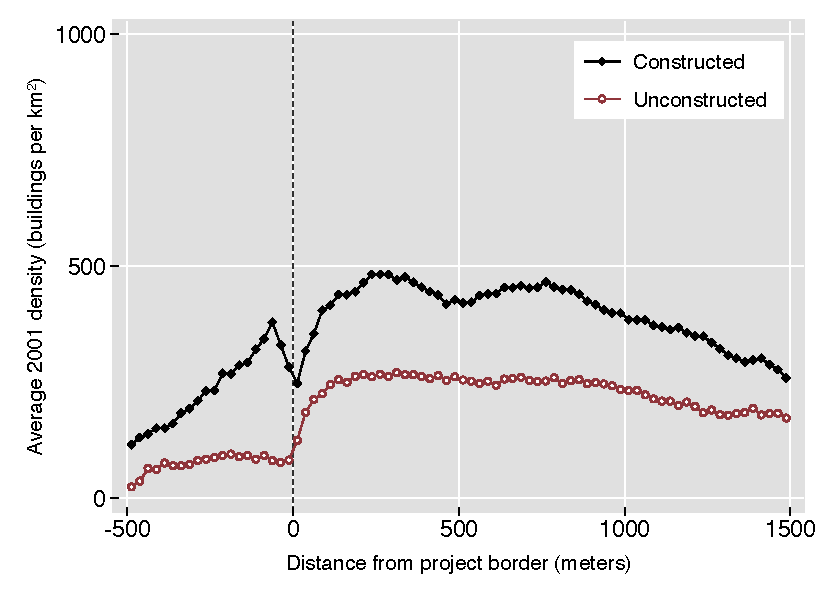
\includegraphics[width=\textwidth,trim={0.3cm .3cm 0.1cm 0cm}, clip=true]{figures/bblu_for_pre_means_4_spk.pdf}

        \end{subfigure}
        \hfill
        \begin{subfigure}[b]{0.48\textwidth}  
                    \caption[]%
            {{\footnotesize \textbf{All Projects} pre-period informal  raw data}}      
            \label{fig:preinf}
            \centering 
            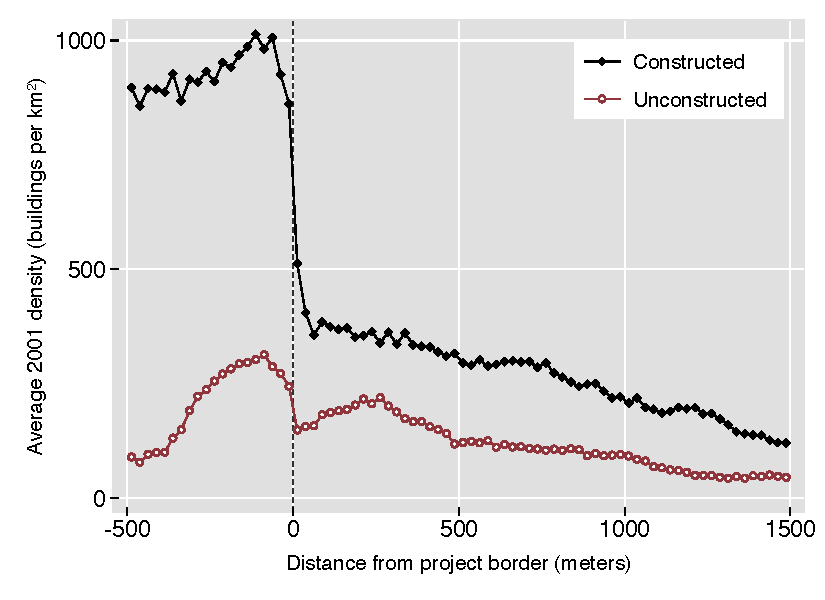
\includegraphics[width=\textwidth,trim={0.3cm .3cm 0.1cm 0cm}, clip=true]{figures/bblu_inf_pre_means_4_spk.pdf}

        \end{subfigure}
        \begin{subfigure}[b]{0.48\textwidth}
                    \caption[Network2]%
            {{\footnotesize \textbf{Greenfield} pre-period formal  raw data}}    
            \label{fig:prefor}
            \centering
            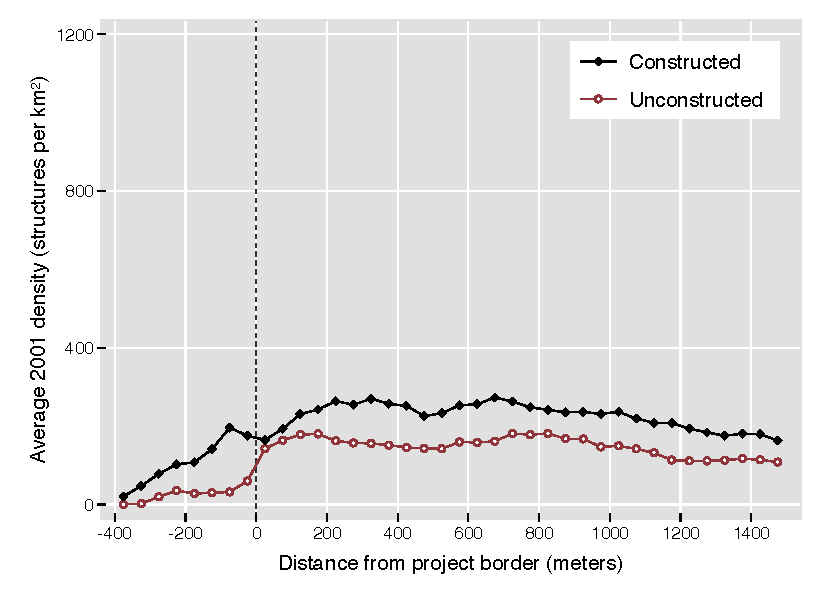
\includegraphics[width=\textwidth,trim={0.3cm .3cm 0.1cm 0cm}, clip=true]{figures/bblu_for_pre_means_4_1_spk.pdf}

        \end{subfigure}
        \hfill
        \begin{subfigure}[b]{0.48\textwidth}  
                    \caption[]%
            {{\footnotesize \textbf{Greenfield} pre-period informal  raw data}}     
            \label{fig:preinf}
            \centering 
            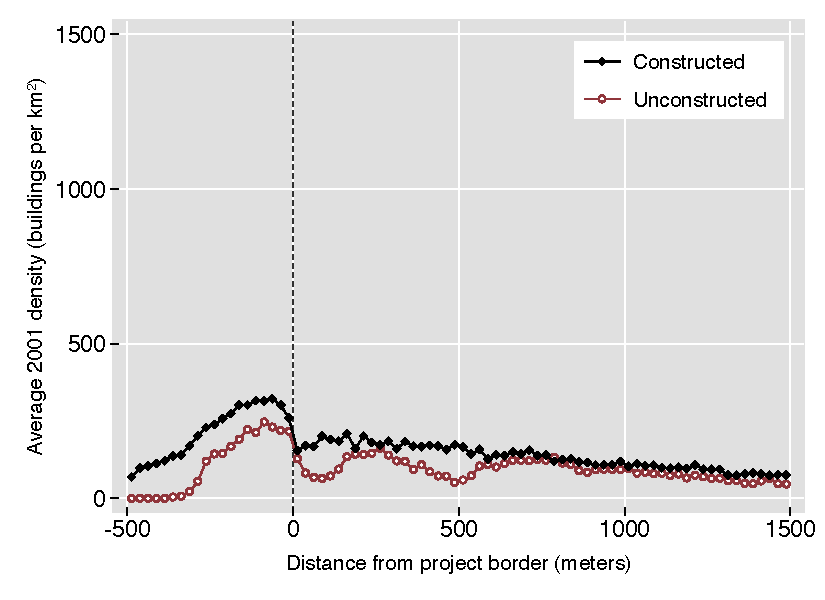
\includegraphics[width=\textwidth,trim={0.3cm .3cm 0.1cm 0cm}, clip=true]{figures/bblu_inf_pre_means_4_1_spk.pdf}

        \end{subfigure}
        \begin{subfigure}[b]{0.48\textwidth}
                    \caption[Network2]%
            {{\footnotesize \textbf{In-Situ} pre-period formal  raw data}}   
            \label{fig:prefor}
            \centering
            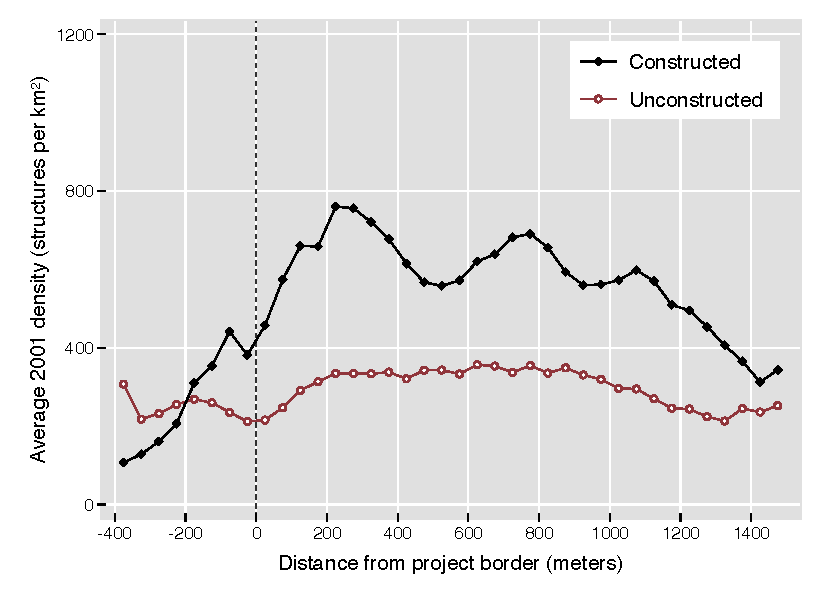
\includegraphics[width=\textwidth,trim={0.3cm .3cm 0.1cm 0cm}, clip=true]{figures/bblu_for_pre_means_4_2_spk.pdf}

        \end{subfigure}
        \hfill
        \begin{subfigure}[b]{0.48\textwidth}  
                    \caption[]%
            {{\footnotesize \textbf{In-Situ} pre-period informal  raw data}}     
            \label{fig:preinf}
            \centering 
            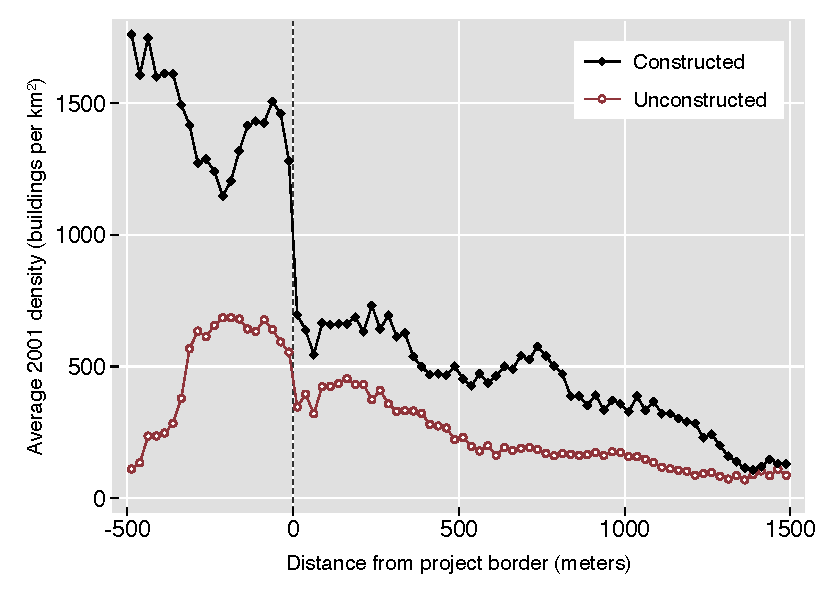
\includegraphics[width=\textwidth,trim={0.3cm .3cm 0.1cm 0cm}, clip=true]{figures/bblu_inf_pre_means_4_2_spk.pdf}

        \end{subfigure}
        \begin{subfigure}[b]{0.48\textwidth}
                    \caption[Network2]%
            {{\footnotesize \textbf{Other} pre-period formal  raw data}}   
            \label{fig:prefor}
            \centering
            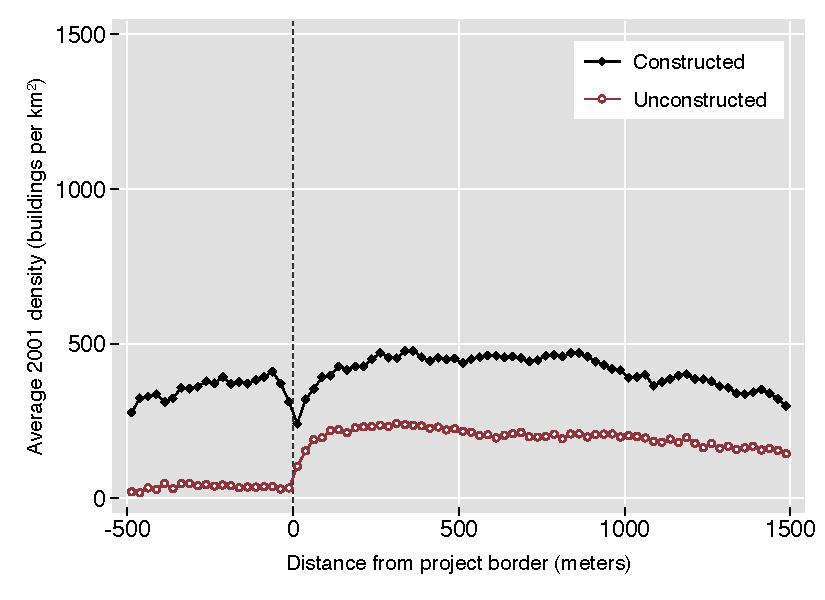
\includegraphics[width=\textwidth,trim={0.3cm .3cm 0.1cm 0cm}, clip=true]{figures/bblu_for_pre_means_4_3_spk.pdf}

        \end{subfigure}
        \hfill
        \begin{subfigure}[b]{0.48\textwidth}  
                    \caption[]%
            {{\footnotesize \textbf{Other} pre-period informal  raw data}}      
            \label{fig:preinf}
            \centering 
            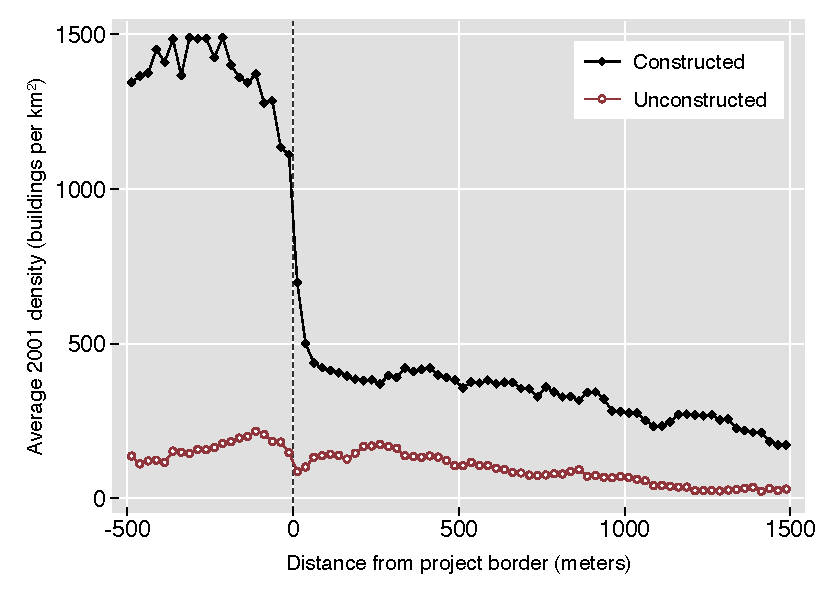
\includegraphics[width=\textwidth,trim={0.3cm .3cm 0.1cm 0cm}, clip=true]{figures/bblu_inf_pre_means_4_3_spk.pdf}

        \end{subfigure}
\end{figure*}


\begin{figure*}
        \centering
   %     \caption[ Pre-Period Housing Densities in Constructed and Unconstructed Projects Areas ]
  %      {\small Pre-Period Densities} 
        %\vspace{2mm}
        \begin{subfigure}[b]{0.48\textwidth}
                    \caption[Network2]%
            {{\footnotesize \textbf{All Projects} pre-period formal fe}}    
            \label{fig:prefor}
            \centering
            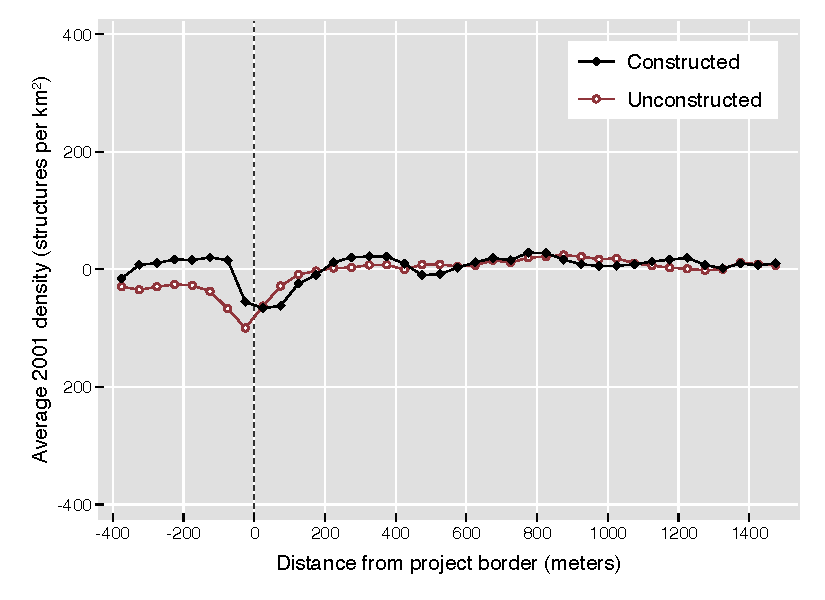
\includegraphics[width=\textwidth,trim={0.3cm .3cm 0.1cm 0cm}, clip=true]{figures/bblu_for_fe_pre_means_4_sp_postk.pdf}

        \end{subfigure}
        \hfill
        \begin{subfigure}[b]{0.48\textwidth}  
                    \caption[]%
            {{\footnotesize \textbf{All Projects} pre-period informal fe }}      
            \label{fig:preinf}
            \centering 
            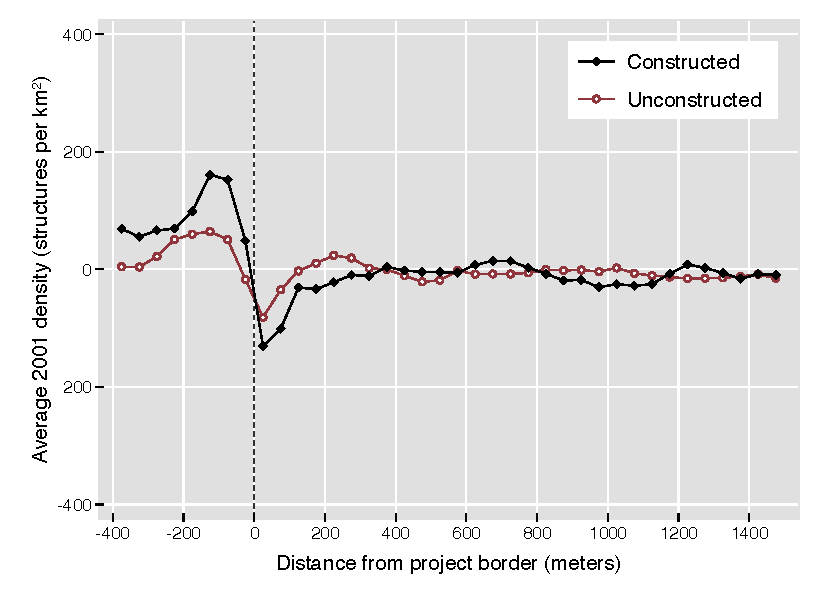
\includegraphics[width=\textwidth,trim={0.3cm .3cm 0.1cm 0cm}, clip=true]{figures/bblu_inf_fe_pre_means_4_sp_postk.pdf}

        \end{subfigure}
        \begin{subfigure}[b]{0.48\textwidth}
                    \caption[Network2]%
            {{\footnotesize \textbf{Greenfield} pre-period formal  fe }}    
            \label{fig:prefor}
            \centering
            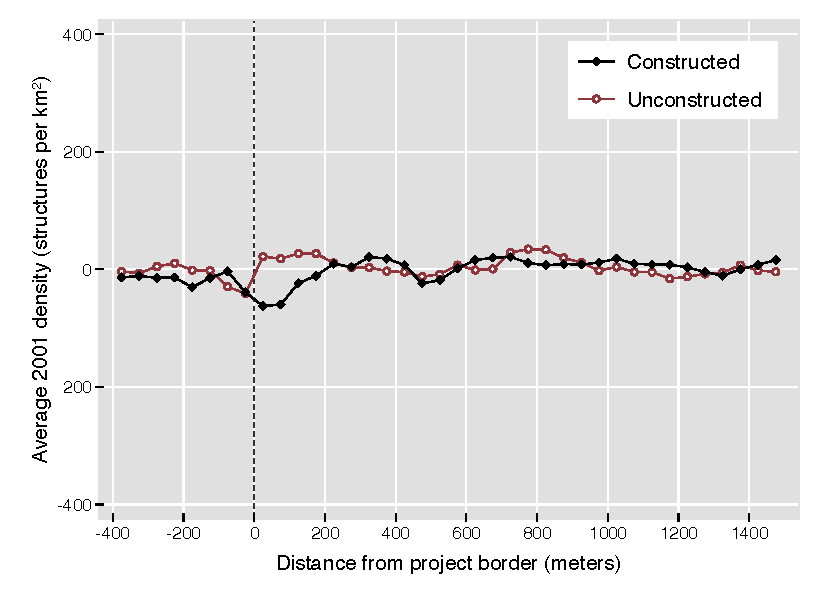
\includegraphics[width=\textwidth,trim={0.3cm .3cm 0.1cm 0cm}, clip=true]{figures/bblu_for_fe_pre_means_4_1_sp_postk.pdf}

        \end{subfigure}
        \hfill
        \begin{subfigure}[b]{0.48\textwidth}  
                    \caption[]%
            {{\footnotesize \textbf{Greenfield} pre-period informal fe }}     
            \label{fig:preinf}
            \centering 
            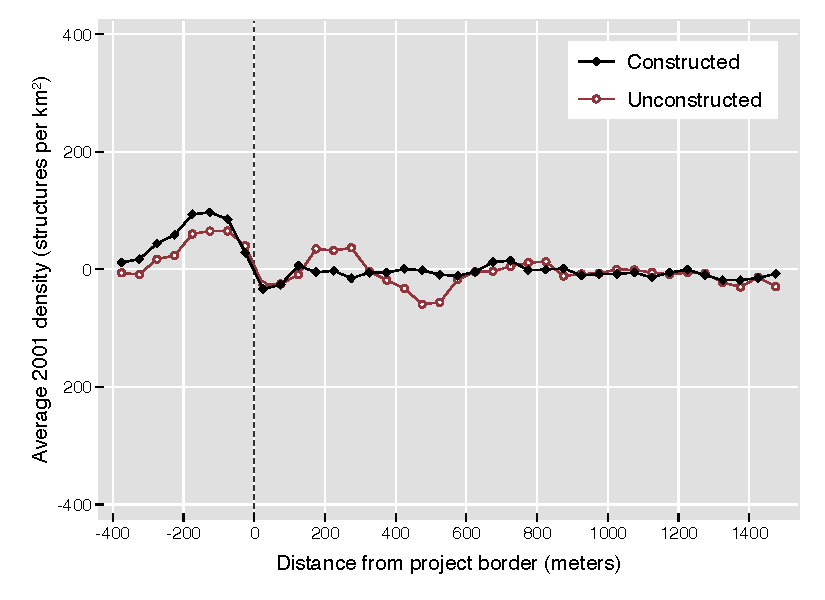
\includegraphics[width=\textwidth,trim={0.3cm .3cm 0.1cm 0cm}, clip=true]{figures/bblu_inf_fe_pre_means_4_1_sp_postk.pdf}

        \end{subfigure}
        \begin{subfigure}[b]{0.48\textwidth}
                    \caption[Network2]%
            {{\footnotesize \textbf{In-Situ} pre-period formal fe }}   
            \label{fig:prefor}
            \centering
            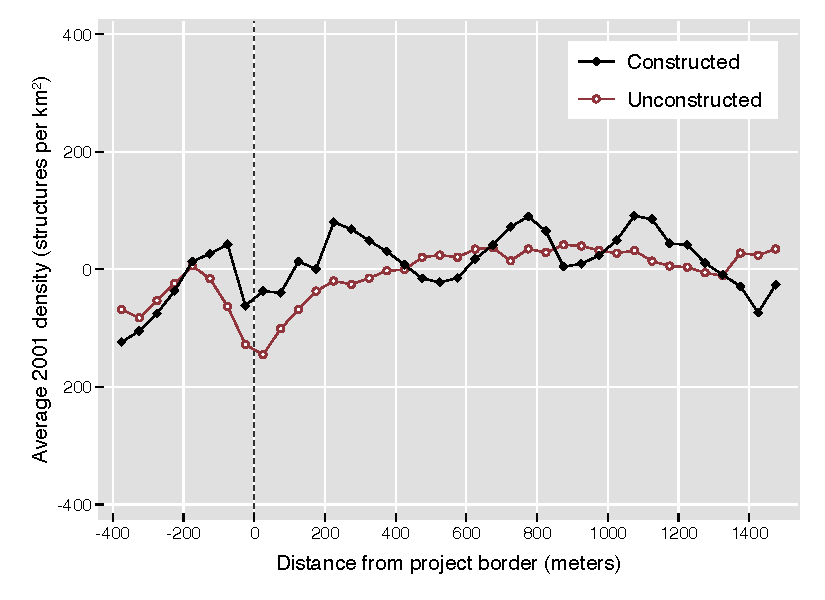
\includegraphics[width=\textwidth,trim={0.3cm .3cm 0.1cm 0cm}, clip=true]{figures/bblu_for_fe_pre_means_4_2_sp_postk.pdf}

        \end{subfigure}
        \hfill
        \begin{subfigure}[b]{0.48\textwidth}  
                    \caption[]%
            {{\footnotesize \textbf{In-Situ} pre-period informal fe }}     
            \label{fig:preinf}
            \centering 
            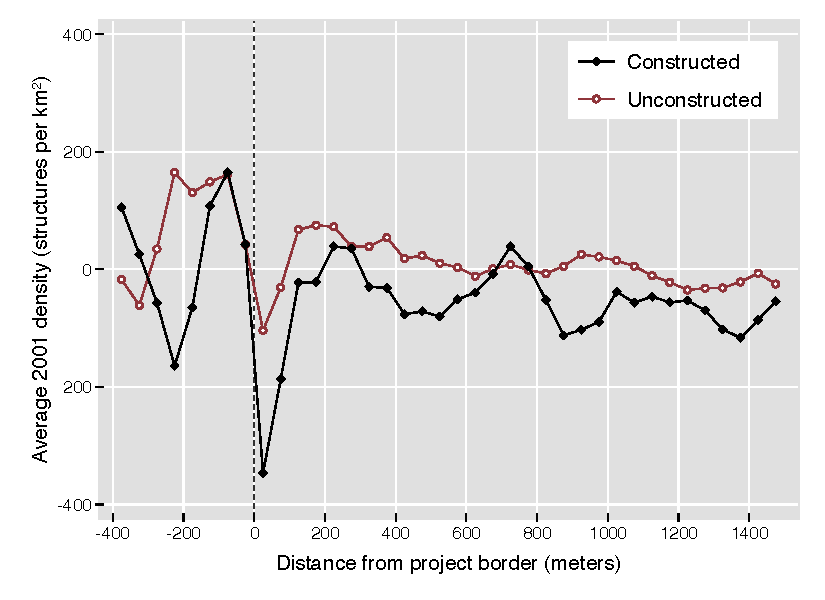
\includegraphics[width=\textwidth,trim={0.3cm .3cm 0.1cm 0cm}, clip=true]{figures/bblu_inf_fe_pre_means_4_2_sp_postk.pdf}

        \end{subfigure}
        \begin{subfigure}[b]{0.48\textwidth}
                    \caption[Network2]%
            {{\footnotesize \textbf{Other} pre-period formal fe }}   
            \label{fig:prefor}
            \centering
            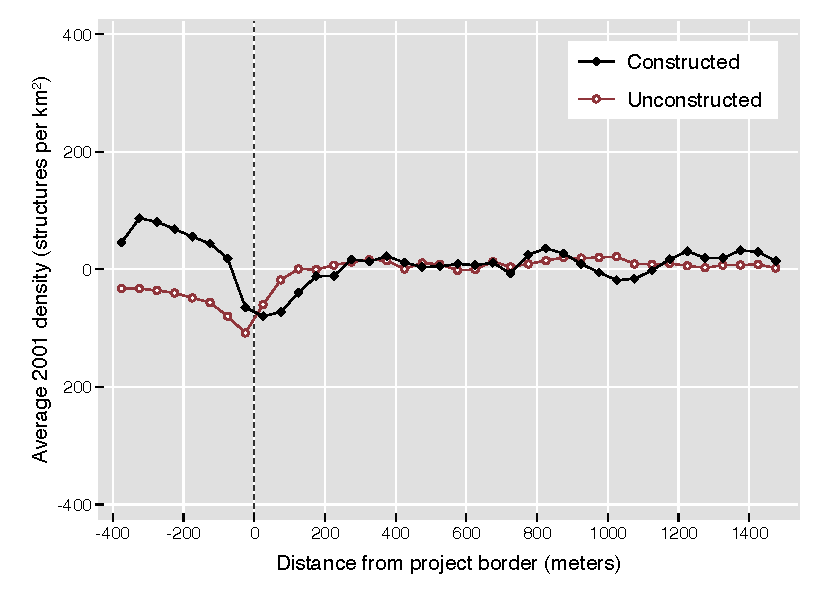
\includegraphics[width=\textwidth,trim={0.3cm .3cm 0.1cm 0cm}, clip=true]{figures/bblu_for_fe_pre_means_4_3_sp_postk.pdf}

        \end{subfigure}
        \hfill
        \begin{subfigure}[b]{0.48\textwidth}  
                    \caption[]%
            {{\footnotesize \textbf{Other} pre-period informal fe }}      
            \label{fig:preinf}
            \centering 
            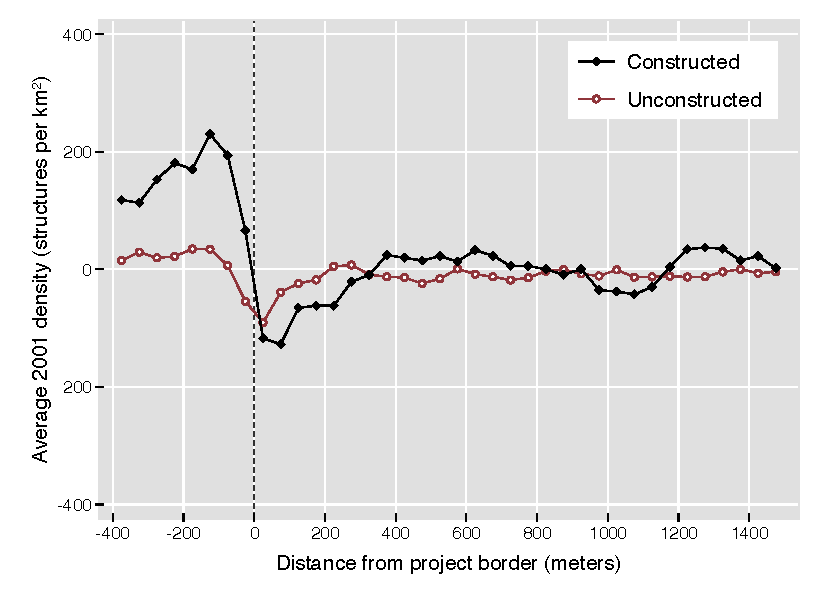
\includegraphics[width=\textwidth,trim={0.3cm .3cm 0.1cm 0cm}, clip=true]{figures/bblu_inf_fe_pre_means_4_3_sp_postk.pdf}

        \end{subfigure}
\end{figure*}








\begin{figure*}
        \centering
   %     \caption[ Pre-Period Housing Densities in Constructed and Unconstructed Projects Areas ]
  %      {\small Pre-Period Densities} 
        %\vspace{2mm}
        \begin{subfigure}[b]{0.48\textwidth}
            \caption[Network2]%
            {{\footnotesize \textbf{All Projects} changes formal raw data}}    
            \label{fig:prefor}
            \centering
            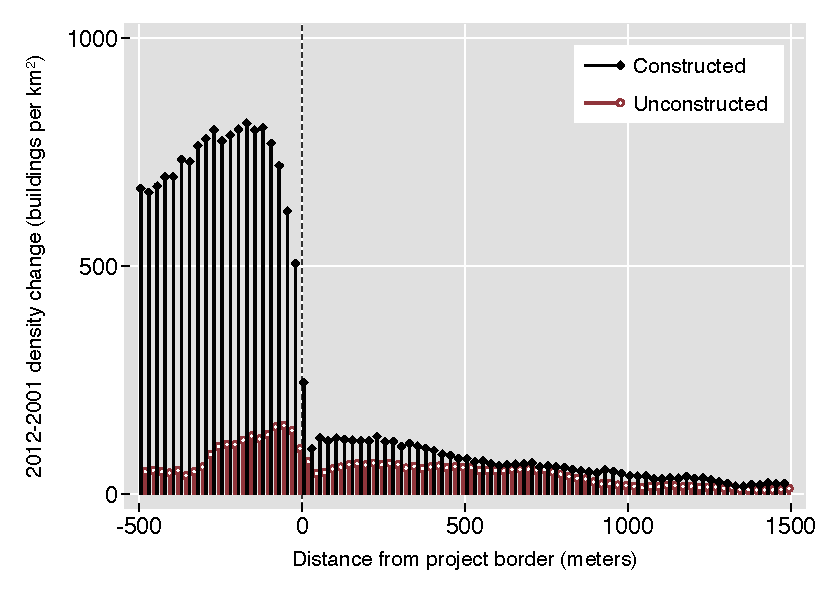
\includegraphics[width=\textwidth,trim={0.3cm .3cm 0.1cm 0cm}, clip=true]{figures/bblu_for_rawchanges_4_spk.pdf}

        \end{subfigure}
        \hfill
        \begin{subfigure}[b]{0.48\textwidth}  
                    \caption[]%
            {{\footnotesize \textbf{All Projects} changes informal  raw data}}      
            \label{fig:preinf}
            \centering 
            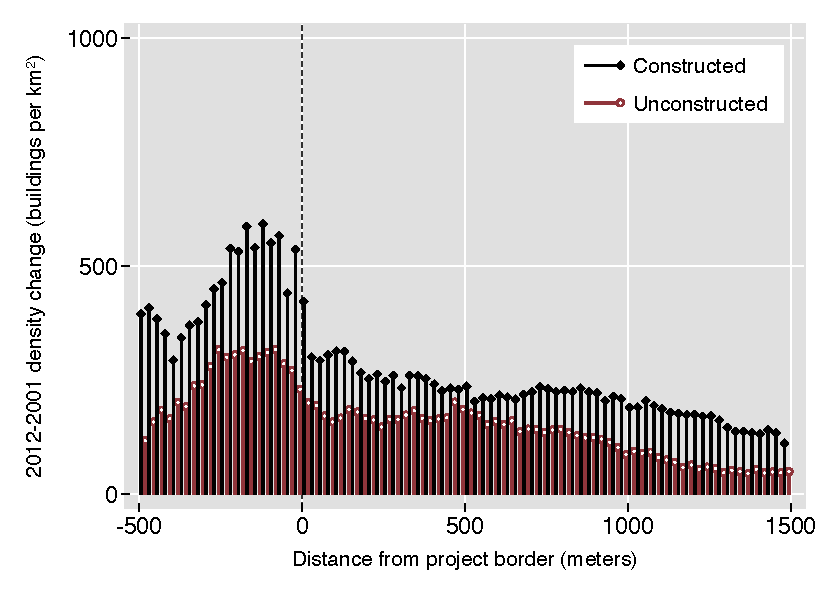
\includegraphics[width=\textwidth,trim={0.3cm .3cm 0.1cm 0cm}, clip=true]{figures/bblu_inf_rawchanges_4_spk.pdf}

        \end{subfigure}
        \begin{subfigure}[b]{0.48\textwidth}
                    \caption[Network2]%
            {{\footnotesize \textbf{Greenfield} changes formal  raw data}}    
            \label{fig:prefor}
            \centering
            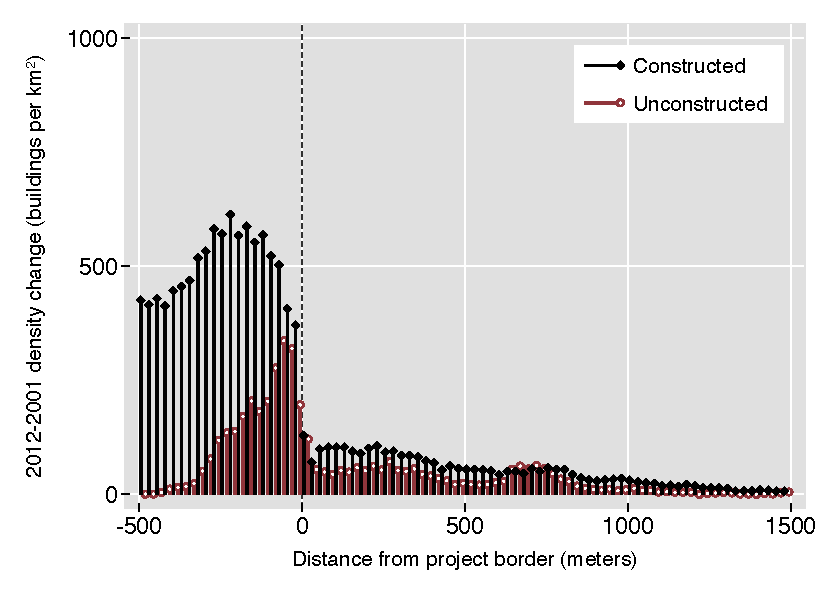
\includegraphics[width=\textwidth,trim={0.3cm .3cm 0.1cm 0cm}, clip=true]{figures/bblu_for_rawchanges_4_1_spk.pdf}

        \end{subfigure}
        \hfill
        \begin{subfigure}[b]{0.48\textwidth}  
                    \caption[]%
            {{\footnotesize \textbf{Greenfield} changes informal raw data }}     
            \label{fig:preinf}
            \centering 
            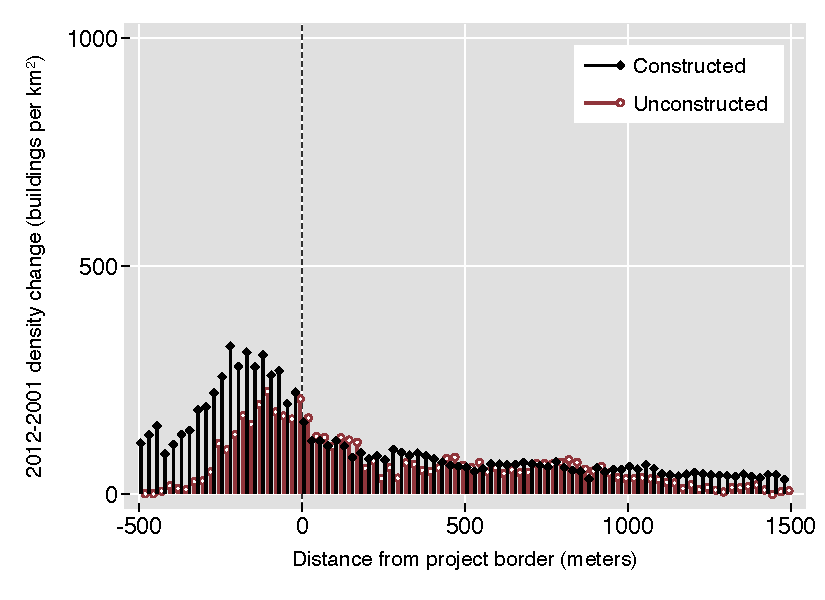
\includegraphics[width=\textwidth,trim={0.3cm .3cm 0.1cm 0cm}, clip=true]{figures/bblu_inf_rawchanges_4_1_spk.pdf}

        \end{subfigure}
        \begin{subfigure}[b]{0.48\textwidth}
                    \caption[Network2]%
            {{\footnotesize \textbf{In-Situ} changes formal raw data }}   
            \label{fig:prefor}
            \centering
            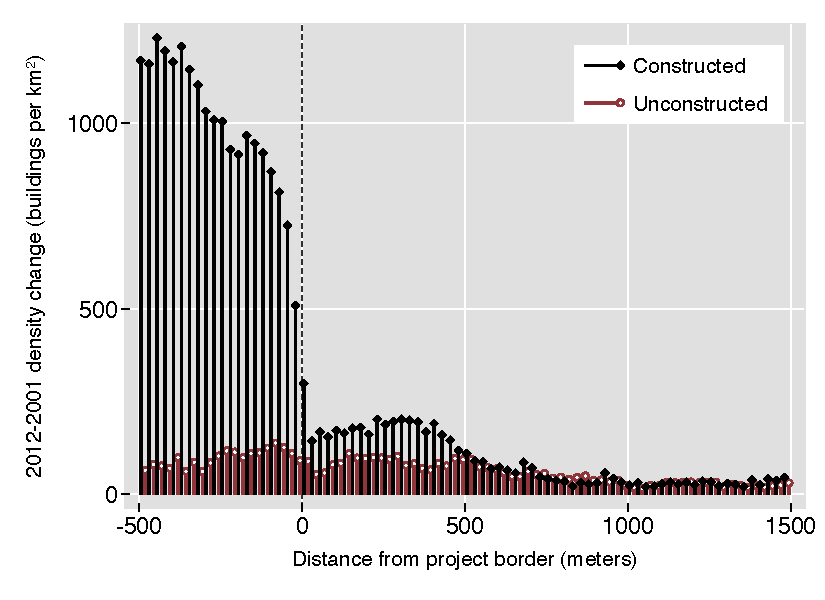
\includegraphics[width=\textwidth,trim={0.3cm .3cm 0.1cm 0cm}, clip=true]{figures/bblu_for_rawchanges_4_2_spk.pdf}

        \end{subfigure}
        \hfill
        \begin{subfigure}[b]{0.48\textwidth}  
                    \caption[]%
            {{\footnotesize \textbf{In-Situ} changes informal raw data }}     
            \label{fig:preinf}
            \centering 
            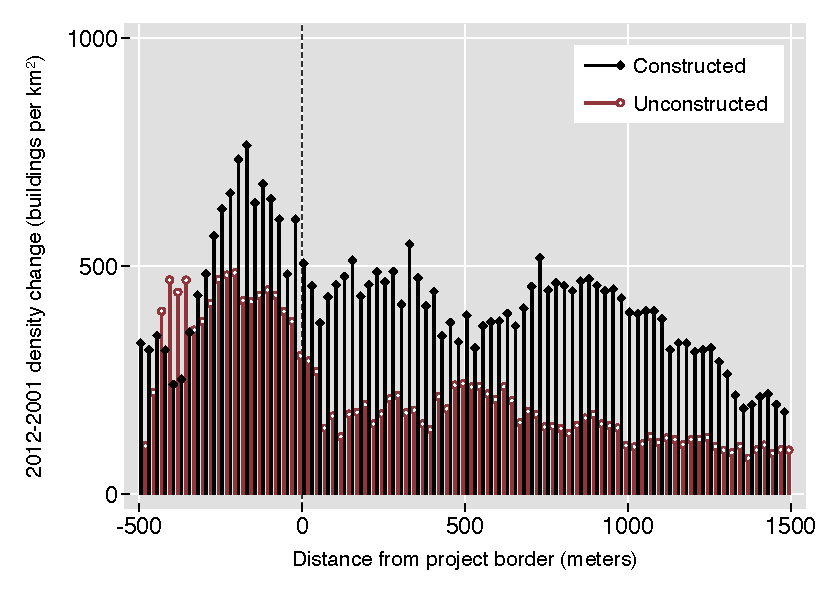
\includegraphics[width=\textwidth,trim={0.3cm .3cm 0.1cm 0cm}, clip=true]{figures/bblu_inf_rawchanges_4_2_spk.pdf}

        \end{subfigure}
        \begin{subfigure}[b]{0.48\textwidth}
                    \caption[Network2]%
            {{\footnotesize \textbf{Other} changes formal raw data}}   
            \label{fig:prefor}
            \centering
            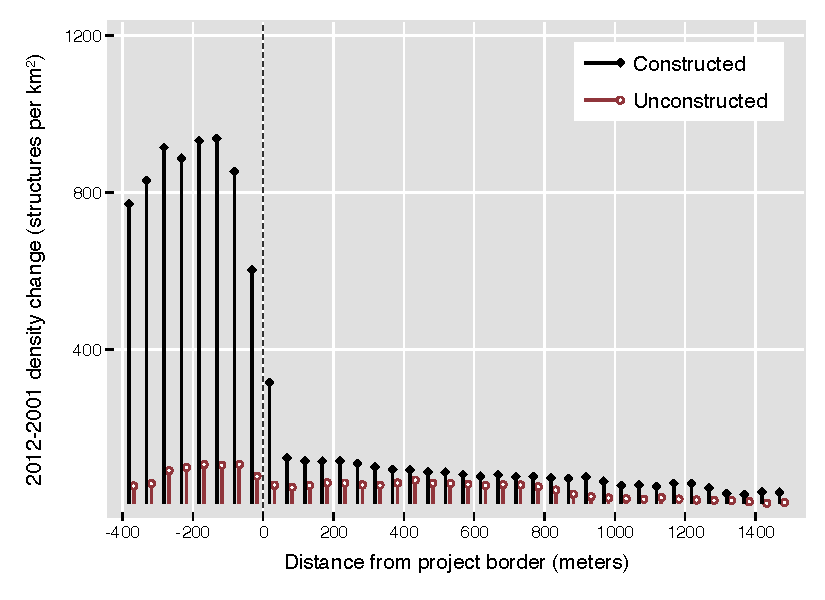
\includegraphics[width=\textwidth,trim={0.3cm .3cm 0.1cm 0cm}, clip=true]{figures/bblu_for_rawchanges_4_3_spk.pdf}

        \end{subfigure}
        \hfill
        \begin{subfigure}[b]{0.48\textwidth} 
                    \caption[]%
            {{\footnotesize \textbf{Other} changes informal  raw data}}      
            \label{fig:preinf} 
            \centering 
            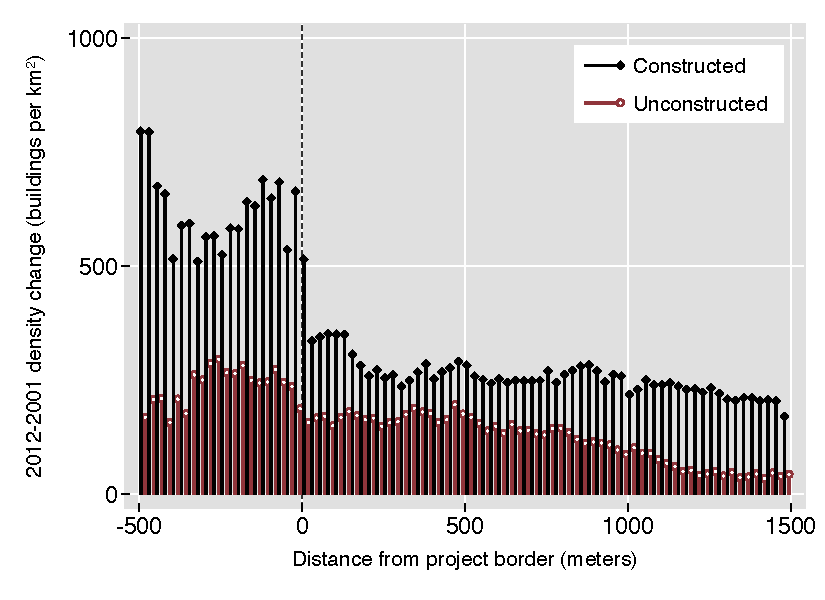
\includegraphics[width=\textwidth,trim={0.3cm .3cm 0.1cm 0cm}, clip=true]{figures/bblu_inf_rawchanges_4_3_spk.pdf}

        \end{subfigure}
\end{figure*}




\begin{figure*}
        \centering
   %     \caption[ Pre-Period Housing Densities in Constructed and Unconstructed Projects Areas ]
  %      {\small Pre-Period Densities} 
        %\vspace{2mm}
        \begin{subfigure}[b]{0.48\textwidth}
            \caption[Network2]%
            {{\footnotesize \textbf{All Projects} changes formal fe }}    
            \label{fig:prefor}
            \centering
            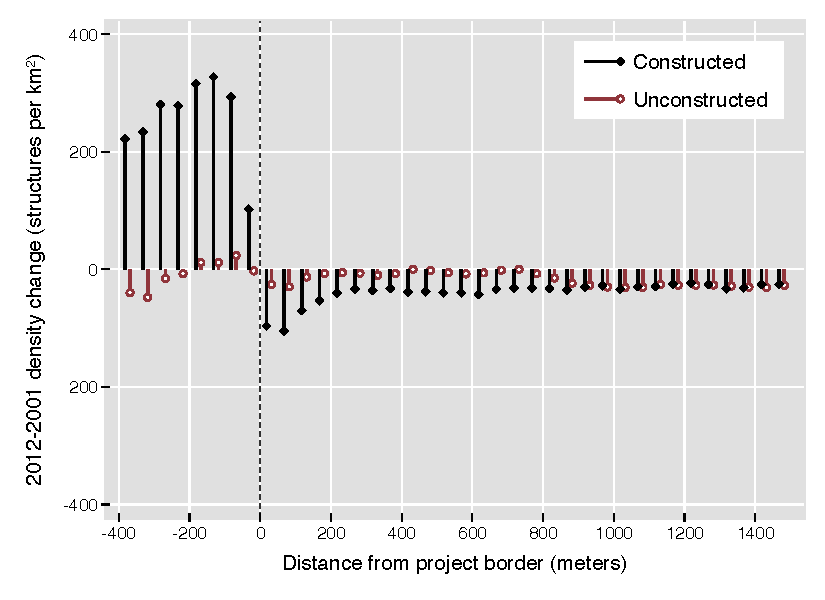
\includegraphics[width=\textwidth,trim={0.3cm .3cm 0.1cm 0cm}, clip=true]{figures/bblu_for_fe_rawchanges_4_sp_postk.pdf}

        \end{subfigure}
        \hfill
        \begin{subfigure}[b]{0.48\textwidth}  
                    \caption[]%
            {{\footnotesize \textbf{All Projects} changes informal  fe }}      
            \label{fig:preinf}
            \centering 
            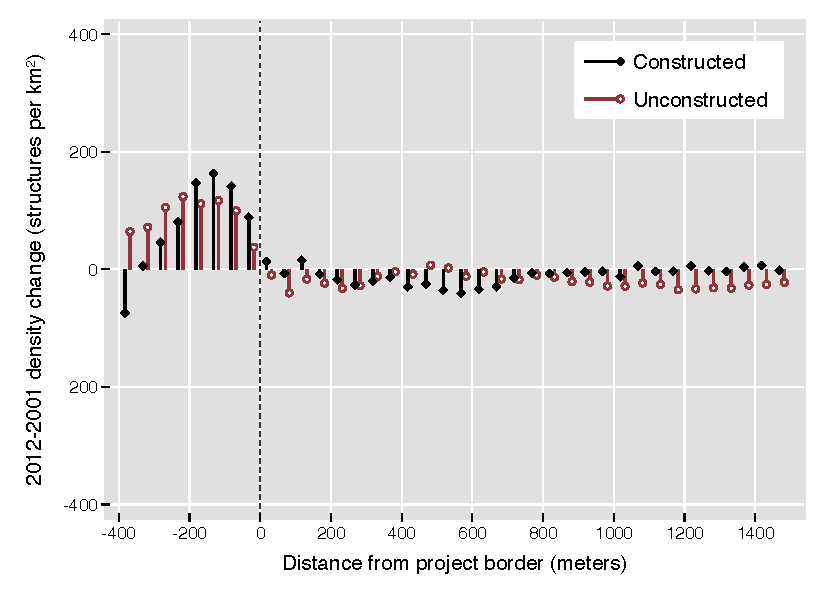
\includegraphics[width=\textwidth,trim={0.3cm .3cm 0.1cm 0cm}, clip=true]{figures/bblu_inf_fe_rawchanges_4_sp_postk.pdf}

        \end{subfigure}
        \begin{subfigure}[b]{0.48\textwidth}
                    \caption[Network2]%
            {{\footnotesize \textbf{Greenfield} changes formal  fe}}    
            \label{fig:prefor}
            \centering
            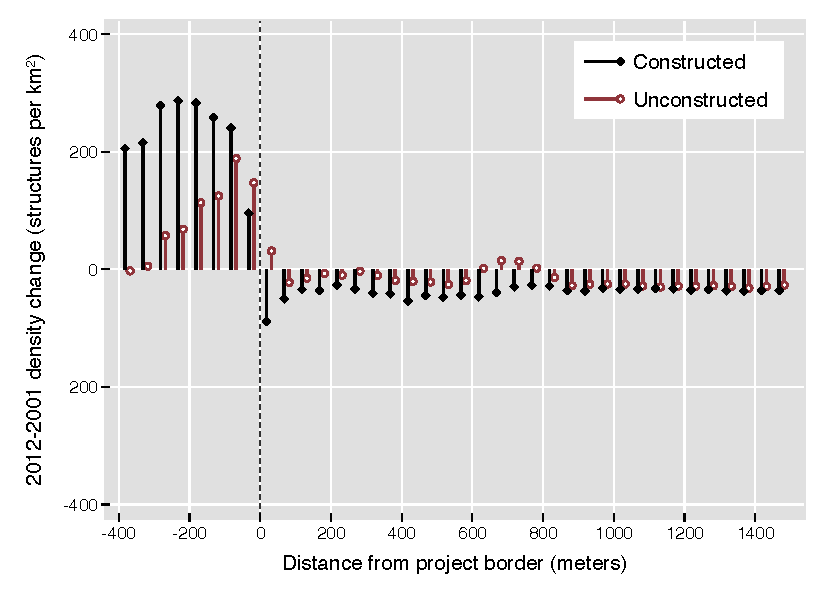
\includegraphics[width=\textwidth,trim={0.3cm .3cm 0.1cm 0cm}, clip=true]{figures/bblu_for_fe_rawchanges_4_1_sp_postk.pdf}

        \end{subfigure}
        \hfill
        \begin{subfigure}[b]{0.48\textwidth}  
                    \caption[]%
            {{\footnotesize \textbf{Greenfield} changes informal fe}}     
            \label{fig:preinf}
            \centering 
            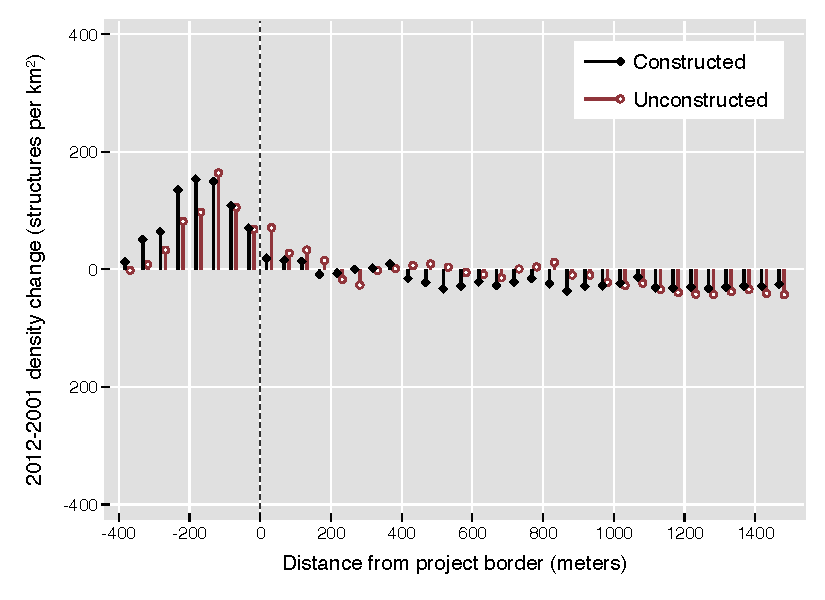
\includegraphics[width=\textwidth,trim={0.3cm .3cm 0.1cm 0cm}, clip=true]{figures/bblu_inf_fe_rawchanges_4_1_sp_postk.pdf}

        \end{subfigure}
        \begin{subfigure}[b]{0.48\textwidth}
                    \caption[Network2]%
            {{\footnotesize \textbf{In-Situ} changes formal fe}}   
            \label{fig:prefor}
            \centering
            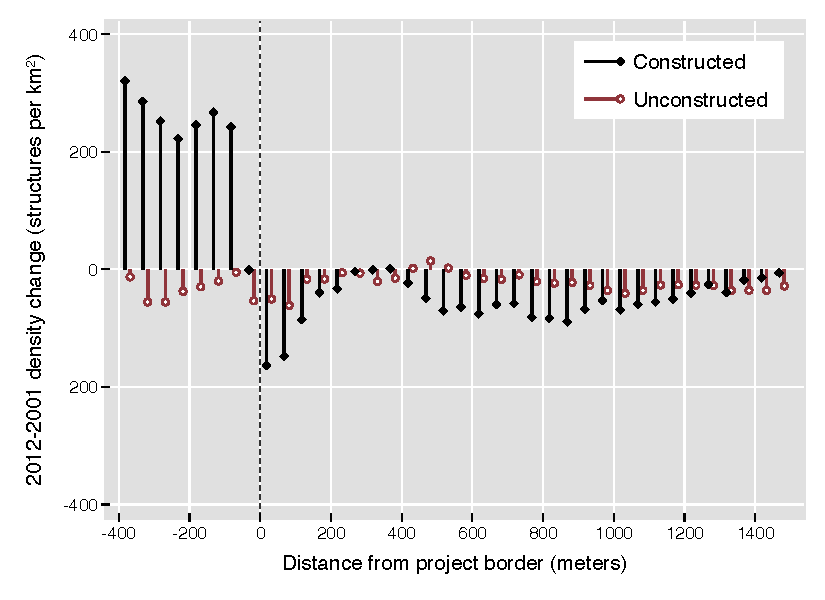
\includegraphics[width=\textwidth,trim={0.3cm .3cm 0.1cm 0cm}, clip=true]{figures/bblu_for_fe_rawchanges_4_2_sp_postk.pdf}

        \end{subfigure}
        \hfill
        \begin{subfigure}[b]{0.48\textwidth}  
                    \caption[]%
            {{\footnotesize \textbf{In-Situ} changes informal fe}}     
            \label{fig:preinf}
            \centering 
            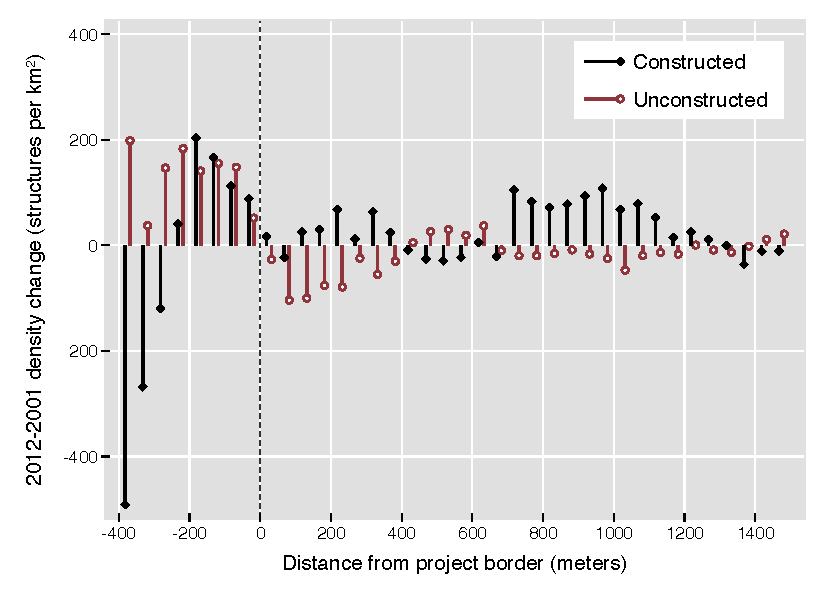
\includegraphics[width=\textwidth,trim={0.3cm .3cm 0.1cm 0cm}, clip=true]{figures/bblu_inf_fe_rawchanges_4_2_sp_postk.pdf}

        \end{subfigure}
        \begin{subfigure}[b]{0.48\textwidth}
                    \caption[Network2]%
            {{\footnotesize \textbf{Other} changes formal fe}}   
            \label{fig:prefor}
            \centering
            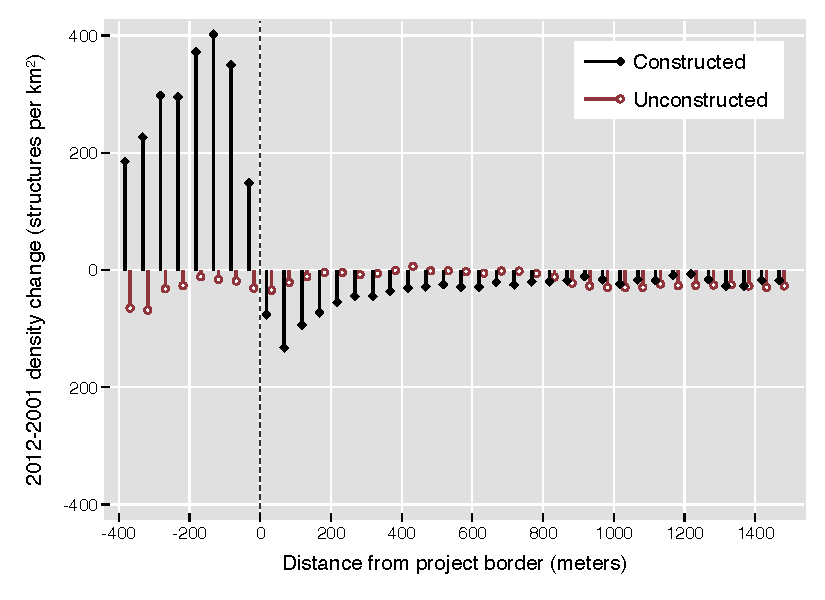
\includegraphics[width=\textwidth,trim={0.3cm .3cm 0.1cm 0cm}, clip=true]{figures/bblu_for_fe_rawchanges_4_3_sp_postk.pdf}

        \end{subfigure}
        \hfill
        \begin{subfigure}[b]{0.48\textwidth} 
                    \caption[]%
            {{\footnotesize \textbf{Other} changes informal  fe}}      
            \label{fig:preinf} 
            \centering 
            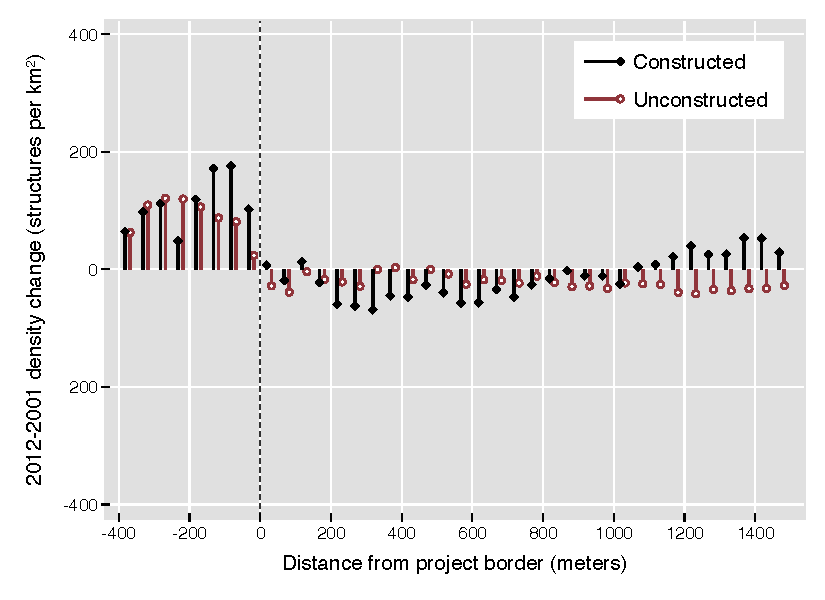
\includegraphics[width=\textwidth,trim={0.3cm .3cm 0.1cm 0cm}, clip=true]{figures/bblu_inf_fe_rawchanges_4_3_sp_postk.pdf}

        \end{subfigure}
\end{figure*}







\begin{table}
\caption{Building Density}
\begin{tabular}{lDDDDD}
\toprule
 & \small (1) & \small (2)  & \small (3) & \small (4) & \small (5) \\
 & Total & Formal  & Informal & Informal Bkyd. & Informal Non-Bkyd. \\ \midrule
\textbf{All Projects} \\inside project      &     448.713\textsuperscript{a}&     436.282\textsuperscript{a}&      12.432                   &     248.895\textsuperscript{a}&    -236.464\textsuperscript{a}\\
                    &   (140.073)                   &    (70.436)                   &   (101.175)                   &    (88.631)                   &    (71.478)                   \\[0.5em]
0-500m outside project &      -4.336                   &      -0.088                   &      -4.248                   &     -27.599                   &      23.352                   \\
                    &    (35.266)                   &    (15.866)                   &    (29.894)                   &    (25.640)                   &    (19.258)                   \\[0.5em]
R$^2$               &       0.442                   &       0.409                   &       0.405                   &       0.387                   &       0.346                   \\

\midrule
\textbf{Greenfield} \\   inside project      &     293.837\textsuperscript{c}&     226.526\textsuperscript{b}&      67.311                   &      98.962                   &     -31.651                   \\
                    &   (176.672)                   &   (111.144)                   &    (83.579)                   &    (80.793)                   &    (39.644)                   \\[0.01em]
0-500m outside project &      -7.412                   &     -10.570                   &       3.158                   &     -24.898                   &      28.056                   \\
                    &    (35.472)                   &    (16.130)                   &    (26.779)                   &    (18.298)                   &    (21.010)                   \\[0.8em] 
\textbf{In-Situ Upgrading} \\   inside project      &     260.276                   &     594.857\textsuperscript{a}&    -334.581                   &      63.220                   &    -397.801                   \\
                    &   (614.381)                   &   (166.178)                   &   (502.699)                   &   (427.884)                   &   (318.117)                   \\[0.01em]
0-500m outside project &      85.438                   &      71.320                   &      14.118                   &     -72.174                   &      86.291                   \\
                    &   (177.751)                   &    (68.889)                   &   (146.296)                   &   (137.790)                   &    (95.302)                   \\[0.8em]
\textbf{Other} \\   inside project      &     705.121\textsuperscript{a}&     600.400\textsuperscript{a}&     104.721                   &     464.361\textsuperscript{a}&    -359.640\textsuperscript{a}\\
                    &   (136.756)                   &    (71.122)                   &   (103.868)                   &   (103.802)                   &    (87.817)                   \\[0.01em]
0-500m outside project &     -35.843                   &       0.982                   &     -36.826                   &     -31.049                   &      -5.777                   \\
                    &    (49.731)                   &    (19.928)                   &    (43.451)                   &    (36.212)                   &    (21.598)                   \\[0.8em]
Mean Outcome 2001   &      526.22                   &      261.56                   &      264.66                   &       96.43                   &      168.23                   \\
Mean Outcome 2011   &      838.62                   &      385.14                   &      453.48                   &      286.79                   &      166.69                   \\
R$^2$               &       0.443                   &       0.411                   &       0.406                   &       0.388                   &       0.347                   \\
N                   &   1,705,534                   &   1,705,534                   &   1,705,534                   &   1,705,534                   &   1,705,534                   \\

\bottomrule
\end{tabular}
\end{table}





\begin{table}[h!] 
\caption{Effect of Housing Projects on Socio-demographics}
\label{table:sorting}
\small
\centering
%\caption{Census Composition Estimates }
\vspace{-2mm}
\begin{tabular}{lDDDDD}
\toprule
& \small (1) & \small (2) & \small (3) & \small (4)& \small (5)\\
& \small Age & \small P.O.B. not Gauteng & \small Unemployed & \small Years of Education & \small Monthly Income \\ \midrule 
\textbf{All Projects} \\inside project      &      -0.166                   &       0.006                   &      -0.046\textsuperscript{b}&       0.155                   &     731.831                   \\
                    &     (0.397)                   &     (0.023)                   &     (0.021)                   &     (0.160)                   &   (553.388)                   \\[0.5em]
0-500m outside project &      -0.010                   &       0.003                   &      -0.019                   &      -0.000                   &     -31.153                   \\
                    &     (0.274)                   &     (0.014)                   &     (0.016)                   &     (0.097)                   &   (366.624)                   \\[0.5em]
R$^2$               &       0.702                   &       0.771                   &       0.528                   &       0.692                   &       0.665                   \\

\midrule
\textbf{Greenfield} \\   inside project      &      -0.411                   &      -0.010                   &       0.027                   &       0.575\textsuperscript{c}&    1278.592                   \\
                    &     (0.683)                   &     (0.060)                   &     (0.046)                   &     (0.323)                   &  (1003.572)                   \\[0.01em]
0-500m outside project &      -0.451                   &       0.036                   &       0.037                   &       0.129                   &     475.350                   \\
                    &     (0.770)                   &     (0.029)                   &     (0.039)                   &     (0.202)                   &   (575.204)                   \\[0.8em] 
\textbf{In-Situ Upgrading} \\   inside project      &       0.747                   &       0.070\textsuperscript{c}&      -0.073\textsuperscript{a}&      -0.111                   &    -360.439                   \\
                    &     (0.589)                   &     (0.040)                   &     (0.028)                   &     (0.348)                   &   (940.760)                   \\[0.01em]
0-500m outside project &       0.155                   &       0.004                   &      -0.044\textsuperscript{c}&      -0.093                   &    -970.291                   \\
                    &     (0.309)                   &     (0.024)                   &     (0.026)                   &     (0.198)                   &   (875.287)                   \\[0.8em]
\textbf{Other} \\   inside project      &      -0.229                   &      -0.021                   &      -0.055\textsuperscript{c}&       0.145                   &    1007.662                   \\
                    &     (0.502)                   &     (0.034)                   &     (0.029)                   &     (0.200)                   &   (762.086)                   \\[0.01em]
0-500m outside project &       0.189                   &      -0.005                   &      -0.029                   &      -0.068                   &      92.806                   \\
                    &     (0.381)                   &     (0.022)                   &     (0.019)                   &     (0.120)                   &   (495.652)                   \\[0.8em]
Mean Outcome 2001   &       27.30                   &        0.37                   &        0.47                   &        8.27                   &    2,477.01                   \\
Mean Outcome 2011   &       28.30                   &        0.43                   &        0.33                   &        9.68                   &    4,486.48                   \\
R$^2$               &       0.705                   &       0.773                   &       0.529                   &       0.694                   &       0.668                   \\
N                   &      12,734                   &      12,727                   &      12,724                   &      12,728                   &      12,724                   \\

\bottomrule
\multicolumn{6}{l}{\footnotesize Standard errors clustered at the project level in parenthesis. \textsuperscript{c} p$<$0.10, \textsuperscript{b} p$<$0.05, \textsuperscript{a} p$<$0.01  }\\
\multicolumn{6}{l}{\footnotesize P.O.B. means ``place of birth.''  Monthly income is in Rands.}
\end{tabular}
\end{table}








\begin{landscape}
{\footnotesize

\begin{table}[]
\small
\centering
\caption{Census Household-level Estimates }\label{table:censusestimates}
\vspace{-2mm}
\resizebox{.9\linewidth}{!}{
\begin{tabular}{lDDDDDDDD}
\toprule
 & \small (1) & \small (2)  & \small (3) & \small (4) & \small (5)  & \small (6)  & \small (7) & (8)\\
 & \small Flush Toilet & \small Water Indoors  & \small Electricity Cooking & \small Electricity Heating & \small Electricity Lighting  & \small Number of Rooms  & \small Household Size & Population Density\\ \midrule 
\textbf{All Projects} \\inside project      &       0.072                   &       0.156\textsuperscript{a}&       0.120\textsuperscript{c}&       0.096                   &       0.075                   &       0.199                   &       0.060                   &   -1092.378                   \\
                    &     (0.055)                   &     (0.051)                   &     (0.061)                   &     (0.060)                   &     (0.067)                   &     (0.205)                   &     (0.087)                   &  (1007.565)                   \\[0.5em]
0-500m outside project &      -0.015                   &       0.039                   &      -0.011                   &      -0.012                   &      -0.019                   &      -0.009                   &      -0.046                   &   -1067.549                   \\
                    &     (0.028)                   &     (0.034)                   &     (0.027)                   &     (0.027)                   &     (0.027)                   &     (0.120)                   &     (0.051)                   &  (1143.586)                   \\[0.5em]
R$^2$               &       0.615                   &       0.593                   &       0.668                   &       0.633                   &       0.637                   &       0.675                   &       0.691                   &       0.607                   \\

\midrule
\textbf{Greenfield} \\   inside project      &       0.138                   &       0.113                   &       0.204                   &       0.088                   &       0.175                   &       0.667\textsuperscript{c}&      -0.008                   &    -373.038                   \\
                    &     (0.142)                   &     (0.141)                   &     (0.133)                   &     (0.148)                   &     (0.136)                   &     (0.381)                   &     (0.205)                   &  (2650.827)                   \\[0.01em]
0-500m outside project &      -0.020                   &      -0.005                   &      -0.005                   &       0.010                   &      -0.015                   &       0.097                   &       0.028                   &   -4593.674                   \\
                    &     (0.069)                   &     (0.060)                   &     (0.052)                   &     (0.055)                   &     (0.039)                   &     (0.278)                   &     (0.109)                   &  (3842.958)                   \\[0.8em] 
\textbf{In-Situ Upgrading} \\   inside project      &       0.030                   &       0.097                   &       0.006                   &       0.049                   &      -0.106                   &      -0.147                   &      -0.069                   &   -2084.616                   \\
                    &     (0.111)                   &     (0.087)                   &     (0.128)                   &     (0.107)                   &     (0.135)                   &     (0.316)                   &     (0.145)                   &  (1612.997)                   \\[0.01em]
0-500m outside project &       0.027                   &       0.047                   &      -0.012                   &      -0.034                   &      -0.040                   &      -0.277                   &      -0.051                   &    -396.579                   \\
                    &     (0.063)                   &     (0.065)                   &     (0.056)                   &     (0.053)                   &     (0.059)                   &     (0.198)                   &     (0.094)                   &  (1437.261)                   \\[0.8em]
\textbf{Other} \\   inside project      &       0.064                   &       0.184\textsuperscript{a}&       0.147\textsuperscript{c}&       0.110                   &       0.142                   &       0.211                   &       0.148                   &    -509.342                   \\
                    &     (0.073)                   &     (0.063)                   &     (0.084)                   &     (0.087)                   &     (0.088)                   &     (0.296)                   &     (0.116)                   &  (1140.917)                   \\[0.01em]
0-500m outside project &      -0.049                   &       0.050                   &      -0.022                   &      -0.015                   &      -0.019                   &       0.042                   &      -0.090                   &    -418.067                   \\
                    &     (0.033)                   &     (0.046)                   &     (0.037)                   &     (0.038)                   &     (0.038)                   &     (0.165)                   &     (0.072)                   &   (838.928)                   \\[0.8em]
Mean Outcome 2001   &        0.79                   &        0.35                   &        0.66                   &        0.62                   &        0.77                   &        3.30                   &        3.51                   &    8,566.83                   \\
Mean Outcome 2011   &        0.83                   &        0.54                   &        0.81                   &        0.72                   &        0.82                   &        3.56                   &        3.18                   &    9,823.82                   \\
R$^2$               &       0.625                   &       0.602                   &       0.674                   &       0.639                   &       0.643                   &       0.679                   &       0.694                   &       0.609                   \\
N                   &      12,732                   &      12,732                   &      12,732                   &      12,732                   &      12,732                   &      12,709                   &      12,730                   &      12,734                   \\

\bottomrule
\multicolumn{9}{l}{\footnotesize All regressions include 3km grid Fixed-Effects. Standard errors clustered at the project level in parenthesis. \textsuperscript{c} p$<$0.10,\textsuperscript{b} p$<$0.05,\textsuperscript{a} p$<$0.01 }
\end{tabular}
}
\end{table}

}
\end{landscape}




\begin{table}
\small
\centering
\caption{Triple Difference Estimates on Log-Prices}\label{table:priceDDD_het}
\vspace{-2mm}
\begin{tabular}{lCC}
\toprule
 & \small (1) & \small (2)  \\ \midrule 
 \textbf{All Projects} \\
 inside project      &      -0.166                   &      -0.151                   \\
                    &     (0.272)                   &     (0.267)                   \\[0.5em]
0-500m outside project &      -0.011                   &      -0.005                   \\
                    &     (0.052)                   &     (0.051)                   \\[0.5em]
Lot Size Controls   &                               &  \checkmark                   \\
r2                  &        0.52                   &        0.52                   \\
N                   &      67,751                   &      67,751                   \\

 \midrule
\textbf{Greenfield} \\   inside project      &       0.086                   &      -0.048                   \\
                    &     (0.212)                   &     (0.209)                   \\[0.01em]
0-500m outside project &      -0.013                   &      -0.006                   \\
                    &     (0.148)                   &     (0.146)                   \\[0.8em]
\textbf{In-Situ Upgrading} \\   inside project      &       0.092                   &       0.153                   \\
                    &     (0.339)                   &     (0.308)                   \\[0.01em]
0-500m outside project &      -0.089                   &      -0.086                   \\
                    &     (0.081)                   &     (0.081)                   \\[0.8em]
\textbf{Other} \\   inside project      &      -0.347                   &      -0.303                   \\
                    &     (0.328)                   &     (0.321)                   \\[0.01em]
0-500m outside project &       0.011                   &       0.015                   \\
                    &     (0.076)                   &     (0.075)                   \\[0.8em]
Lot Size Controls   &                               &  \checkmark                   \\
r2                  &        0.52                   &        0.52                   \\
N                   &      67,751                   &      67,751                   \\

\bottomrule
\multicolumn{3}{l}{\footnotesize Standard errors clustered at the project level in parenthesis.} \\
\multicolumn{3}{l}{ \textsuperscript{c} p$<$0.10,\textsuperscript{b} p$<$0.05,\textsuperscript{a} p$<$0.01 }
\end{tabular}
\end{table} 

% \begin{figure}
% 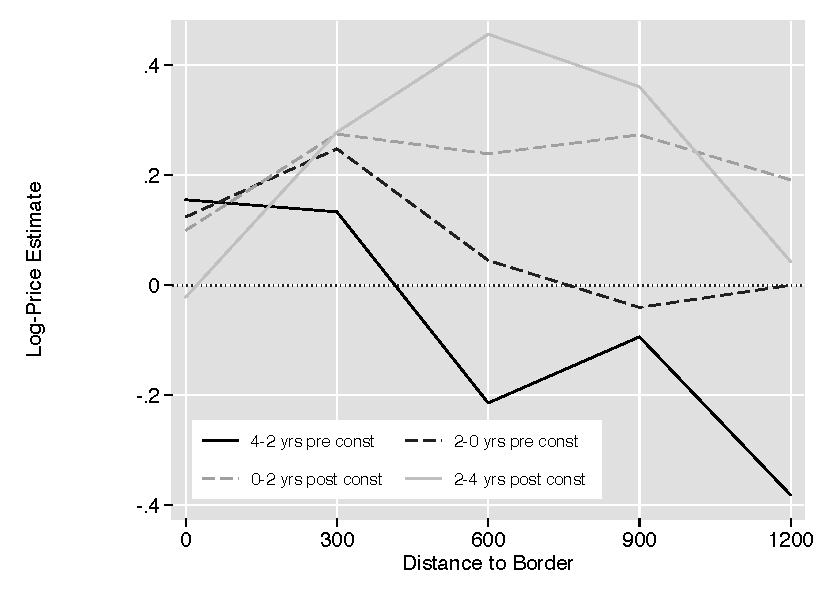
\includegraphics{figures/price_to_event_30.pdf}
% \end{figure}


\end{document}


